\documentclass[12pt, letterpaper, twoside]{article}
\usepackage[utf8]{inputenc}
\usepackage{ mathrsfs }

\usepackage{titlesec}

\usepackage{tikz}
\usetikzlibrary{scopes}

\titlespacing\section{0pt}{12pt plus 4pt minus 2pt}{0pt plus 2pt minus 2pt}
\titlespacing\subsection{0pt}{12pt plus 4pt minus 2pt}{0pt plus 2pt minus 2pt}
\titlespacing\subsubsection{0pt}{12pt plus 4pt minus 2pt}{0pt plus 2pt minus 2pt}


\title{Math 260 Notes}
\author{Zachary Chao}
\date{April 03 2018}

\begin{document}

A $5.6kg$ box has an acceleration of $1.7m/s^2$ when it is pulled by a horizontal force across a surface with $\mu_k = 0.50$. Find the word done over a distance of $14cm$ by the following forces.
\textbf{(a)} the horizontal force
\textbf{(b)} the frictional force
\textbf{(c)} the net force
\textbf{(d)} What is the change in kinetic energy of the box?


\begin{tikzpicture}[
    force/.style={>=latex,draw=blue,fill=blue},
    axis/.style={densely dashed,gray,font=\small},
    M/.style={rectangle,draw,fill=lightgray,minimum size=0.5cm,thin},
    m/.style={rectangle,draw=black,fill=lightgray,minimum size=0.3cm,thin},
    plane/.style={draw=black,fill=blue!10},
    string/.style={draw=red, thick},
    pulley/.style={thick},
]

\matrix[column sep=1cm] {
    \node[m] (m) {};
    {[force,->]
        \draw (m.north) -- ++(0,1) node[above] {$F_N$};
        \draw (m.south) -- ++(0,-1) node[below] {$F_g$};
        \draw (m.east) -- ++(.7,0) node[right] {$F$};
        \draw (m.west) -- +(-.5,0) node[left] {$F_k$};
    }
\\
};
\end{tikzpicture}

$$F_N = mg, \quad F_g = mg, \quad F = ma, \quad F_k = \mu_k g$$


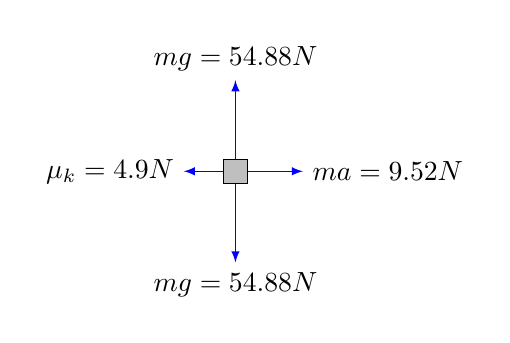
\begin{tikzpicture}[
    force/.style={>=latex,draw=blue,fill=blue},
    axis/.style={densely dashed,gray,font=\small},
    M/.style={rectangle,draw,fill=lightgray,minimum size=0.5cm,thin},
    m/.style={rectangle,draw=black,fill=lightgray,minimum size=0.3cm,thin},
    plane/.style={draw=black,fill=blue!10},
    string/.style={draw=red, thick},
    pulley/.style={thick},
]

\matrix[column sep=1cm] {
    \node[m] (m) {};
    {[force,->]
        \draw (m.north) -- ++(0,1) node[above] {$mg = 54.88N$};
        \draw (m.south) -- ++(0,-1) node[below] {$mg = 54.88N$};
        \draw (m.east) -- ++(.7,0) node[right] {$ma = 9.52N$};
        \draw (m.west) -- +(-.5,0) node[left] {$\mu_k = 4.9N$};
    }
\\
};
\end{tikzpicture}

a, b and c can easily be discerned from the free body diagram.\\
As for d, kinetic energy = $\frac{1}{2}mv^2$. Thus,
$$\Delta KE = \frac{1}{2}m \Delta v^2$$

As we have distance and acceleration, finding the change in velocity can be found using, 
$$v_f^2 = 2ad$$
$$v_f = \sqrt{2ad}$$
$$v_f = 0.476m/s$$
$$KE = 0.6344$$

\end{document}




